\documentclass[1p]{elsarticle_modified}
%\bibliographystyle{elsarticle-num}

%\usepackage[colorlinks]{hyperref}
%\usepackage{abbrmath_seonhwa} %\Abb, \Ascr, \Acal ,\Abf, \Afrak
\usepackage{amsfonts}
\usepackage{amssymb}
\usepackage{amsmath}
\usepackage{amsthm}
\usepackage{scalefnt}
\usepackage{amsbsy}
\usepackage{kotex}
\usepackage{caption}
\usepackage{subfig}
\usepackage{color}
\usepackage{graphicx}
\usepackage{xcolor} %% white, black, red, green, blue, cyan, magenta, yellow
\usepackage{float}
\usepackage{setspace}
\usepackage{hyperref}

\usepackage{tikz}
\usetikzlibrary{arrows}

\usepackage{multirow}
\usepackage{array} % fixed length table
\usepackage{hhline}

%%%%%%%%%%%%%%%%%%%%%
\makeatletter
\renewcommand*\env@matrix[1][\arraystretch]{%
	\edef\arraystretch{#1}%
	\hskip -\arraycolsep
	\let\@ifnextchar\new@ifnextchar
	\array{*\c@MaxMatrixCols c}}
\makeatother %https://tex.stackexchange.com/questions/14071/how-can-i-increase-the-line-spacing-in-a-matrix
%%%%%%%%%%%%%%%

\usepackage[normalem]{ulem}

\newcommand{\msout}[1]{\ifmmode\text{\sout{\ensuremath{#1}}}\else\sout{#1}\fi}
%SOURCE: \msout is \stkout macro in https://tex.stackexchange.com/questions/20609/strikeout-in-math-mode

\newcommand{\cancel}[1]{
	\ifmmode
	{\color{red}\msout{#1}}
	\else
	{\color{red}\sout{#1}}
	\fi
}

\newcommand{\add}[1]{
	{\color{blue}\uwave{#1}}
}

\newcommand{\replace}[2]{
	\ifmmode
	{\color{red}\msout{#1}}{\color{blue}\uwave{#2}}
	\else
	{\color{red}\sout{#1}}{\color{blue}\uwave{#2}}
	\fi
}

\newcommand{\Sol}{\mathcal{S}} %segment
\newcommand{\D}{D} %diagram
\newcommand{\A}{\mathcal{A}} %arc


%%%%%%%%%%%%%%%%%%%%%%%%%%%%%5 test

\def\sl{\operatorname{\textup{SL}}(2,\Cbb)}
\def\psl{\operatorname{\textup{PSL}}(2,\Cbb)}
\def\quan{\mkern 1mu \triangleright \mkern 1mu}

\theoremstyle{definition}
\newtheorem{thm}{Theorem}[section]
\newtheorem{prop}[thm]{Proposition}
\newtheorem{lem}[thm]{Lemma}
\newtheorem{ques}[thm]{Question}
\newtheorem{cor}[thm]{Corollary}
\newtheorem{defn}[thm]{Definition}
\newtheorem{exam}[thm]{Example}
\newtheorem{rmk}[thm]{Remark}
\newtheorem{alg}[thm]{Algorithm}

\newcommand{\I}{\sqrt{-1}}
\begin{document}

%\begin{frontmatter}
%
%\title{Boundary parabolic representations of knots up to 8 crossings}
%
%%% Group authors per affiliation:
%\author{Yunhi Cho} 
%\address{Department of Mathematics, University of Seoul, Seoul, Korea}
%\ead{yhcho@uos.ac.kr}
%
%
%\author{Seonhwa Kim} %\fnref{s_kim}}
%\address{Center for Geometry and Physics, Institute for Basic Science, Pohang, 37673, Korea}
%\ead{ryeona17@ibs.re.kr}
%
%\author{Hyuk Kim}
%\address{Department of Mathematical Sciences, Seoul National University, Seoul 08826, Korea}
%\ead{hyukkim@snu.ac.kr}
%
%\author{Seokbeom Yoon}
%\address{Department of Mathematical Sciences, Seoul National University, Seoul, 08826,  Korea}
%\ead{sbyoon15@snu.ac.kr}
%
%\begin{abstract}
%We find all boundary parabolic representation of knots up to 8 crossings.
%
%\end{abstract}
%\begin{keyword}
%    \MSC[2010] 57M25 
%\end{keyword}
%
%\end{frontmatter}

%\linenumbers
%\tableofcontents
%
\newcommand\colored[1]{\textcolor{white}{\rule[-0.35ex]{0.8em}{1.4ex}}\kern-0.8em\color{red} #1}%
%\newcommand\colored[1]{\textcolor{white}{ #1}\kern-2.17ex	\textcolor{white}{ #1}\kern-1.81ex	\textcolor{white}{ #1}\kern-2.15ex\color{red}#1	}

{\Large $\underline{12n_{0740}~(K12n_{0740})}$}

\setlength{\tabcolsep}{10pt}
\renewcommand{\arraystretch}{1.6}
\vspace{1cm}\begin{tabular}{m{100pt}>{\centering\arraybackslash}m{274pt}}
\multirow{5}{120pt}{
	\centering
	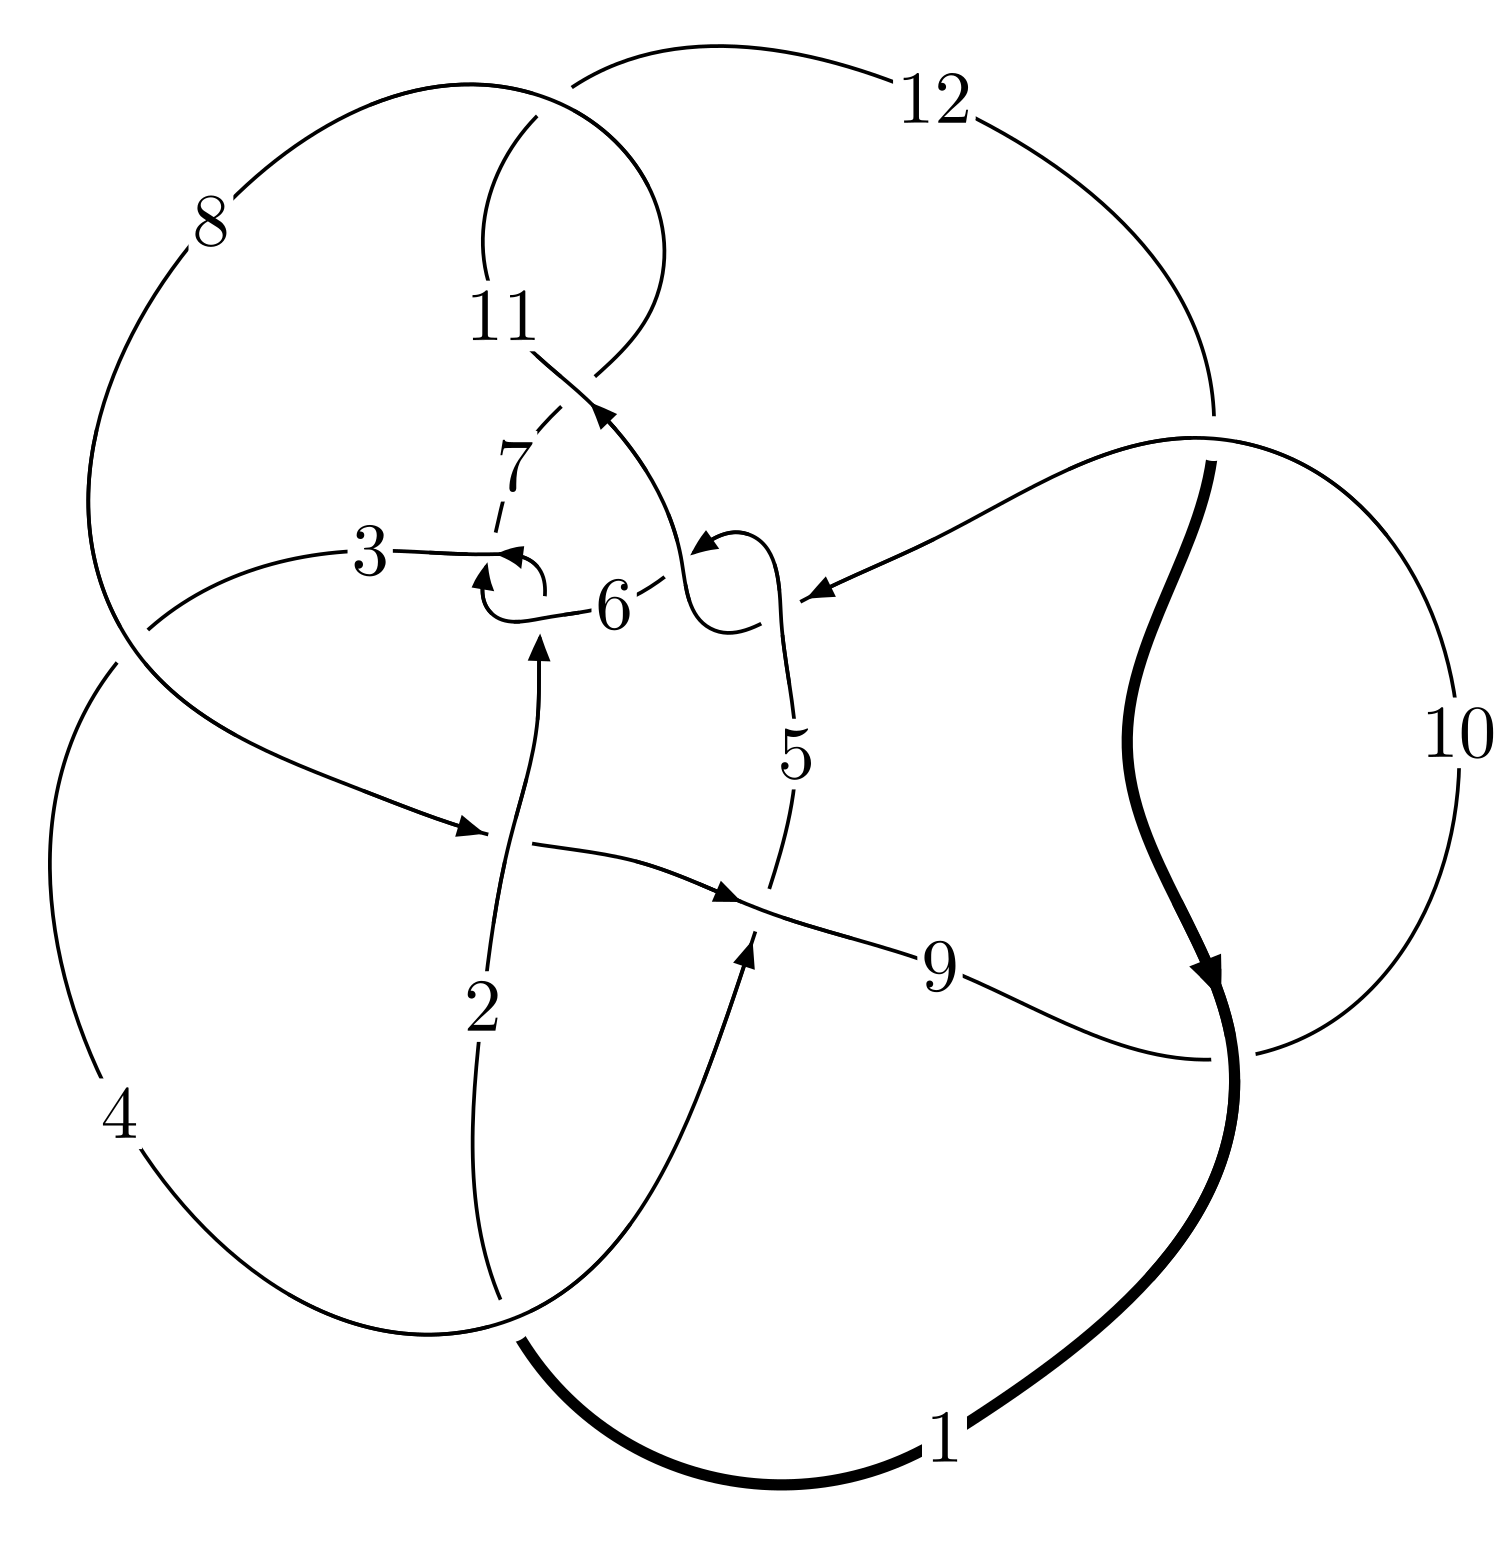
\includegraphics[width=112pt]{../../../GIT/diagram.site/Diagrams/png/2829_12n_0740.png}\\
\ \ \ A knot diagram\footnotemark}&
\allowdisplaybreaks
\textbf{Linearized knot diagam} \\
\cline{2-2}
 &
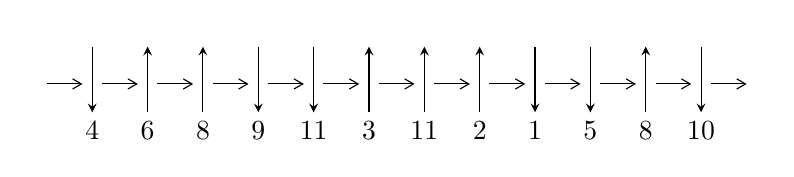
\begin{tikzpicture}[x=20pt, y=17pt]
	% nodes
	\node (C0) at (0, 0) {};
	\node (C1) at (1, 0) {};
	\node (C1U) at (1, +1) {};
	\node (C1D) at (1, -1) {4};

	\node (C2) at (2, 0) {};
	\node (C2U) at (2, +1) {};
	\node (C2D) at (2, -1) {6};

	\node (C3) at (3, 0) {};
	\node (C3U) at (3, +1) {};
	\node (C3D) at (3, -1) {8};

	\node (C4) at (4, 0) {};
	\node (C4U) at (4, +1) {};
	\node (C4D) at (4, -1) {9};

	\node (C5) at (5, 0) {};
	\node (C5U) at (5, +1) {};
	\node (C5D) at (5, -1) {11};

	\node (C6) at (6, 0) {};
	\node (C6U) at (6, +1) {};
	\node (C6D) at (6, -1) {3};

	\node (C7) at (7, 0) {};
	\node (C7U) at (7, +1) {};
	\node (C7D) at (7, -1) {11};

	\node (C8) at (8, 0) {};
	\node (C8U) at (8, +1) {};
	\node (C8D) at (8, -1) {2};

	\node (C9) at (9, 0) {};
	\node (C9U) at (9, +1) {};
	\node (C9D) at (9, -1) {1};

	\node (C10) at (10, 0) {};
	\node (C10U) at (10, +1) {};
	\node (C10D) at (10, -1) {5};

	\node (C11) at (11, 0) {};
	\node (C11U) at (11, +1) {};
	\node (C11D) at (11, -1) {8};

	\node (C12) at (12, 0) {};
	\node (C12U) at (12, +1) {};
	\node (C12D) at (12, -1) {10};
	\node (C13) at (13, 0) {};

	% arrows
	\draw[->,>={angle 60}]
	(C0) edge (C1) (C1) edge (C2) (C2) edge (C3) (C3) edge (C4) (C4) edge (C5) (C5) edge (C6) (C6) edge (C7) (C7) edge (C8) (C8) edge (C9) (C9) edge (C10) (C10) edge (C11) (C11) edge (C12) (C12) edge (C13) ;	\draw[->,>=stealth]
	(C1U) edge (C1D) (C2D) edge (C2U) (C3D) edge (C3U) (C4U) edge (C4D) (C5U) edge (C5D) (C6D) edge (C6U) (C7D) edge (C7U) (C8D) edge (C8U) (C9U) edge (C9D) (C10U) edge (C10D) (C11D) edge (C11U) (C12U) edge (C12D) ;
	\end{tikzpicture} \\
\hhline{~~} \\& 
\textbf{Solving Sequence} \\ \cline{2-2} 
 &
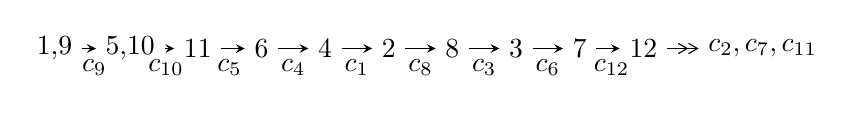
\begin{tikzpicture}[x=23pt, y=7pt]
	% node
	\node (A0) at (-1/8, 0) {1,9};
	\node (A1) at (17/16, 0) {5,10};
	\node (A2) at (17/8, 0) {11};
	\node (A3) at (25/8, 0) {6};
	\node (A4) at (33/8, 0) {4};
	\node (A5) at (41/8, 0) {2};
	\node (A6) at (49/8, 0) {8};
	\node (A7) at (57/8, 0) {3};
	\node (A8) at (65/8, 0) {7};
	\node (A9) at (73/8, 0) {12};
	\node (C1) at (1/2, -1) {$c_{9}$};
	\node (C2) at (13/8, -1) {$c_{10}$};
	\node (C3) at (21/8, -1) {$c_{5}$};
	\node (C4) at (29/8, -1) {$c_{4}$};
	\node (C5) at (37/8, -1) {$c_{1}$};
	\node (C6) at (45/8, -1) {$c_{8}$};
	\node (C7) at (53/8, -1) {$c_{3}$};
	\node (C8) at (61/8, -1) {$c_{6}$};
	\node (C9) at (69/8, -1) {$c_{12}$};
	\node (A10) at (11, 0) {$c_{2},c_{7},c_{11}$};

	% edge
	\draw[->,>=stealth]	
	(A0) edge (A1) (A1) edge (A2) (A2) edge (A3) (A3) edge (A4) (A4) edge (A5) (A5) edge (A6) (A6) edge (A7) (A7) edge (A8) (A8) edge (A9) ;
	\draw[->>,>={angle 60}]	
	(A9) edge (A10);
\end{tikzpicture} \\ 

\end{tabular} \\

\footnotetext{
The image of knot diagram is generated by the software ``\textbf{Draw programme}" developed by Andrew Bartholomew(\url{http://www.layer8.co.uk/maths/draw/index.htm\#Running-draw}), where we modified some parts for our purpose(\url{https://github.com/CATsTAILs/LinksPainter}).
}\phantom \\ \newline 
\centering \textbf{Ideals for irreducible components\footnotemark of $X_{\text{par}}$} 
 
\begin{align*}
I^u_{1}&=\langle 
1.79550\times10^{17} u^{29}+2.44036\times10^{18} u^{28}+\cdots+5.15180\times10^{17} b-1.38475\times10^{18},\\
\phantom{I^u_{1}}&\phantom{= \langle  }-2.66097\times10^{17} u^{29}-3.83157\times10^{18} u^{28}+\cdots+5.15180\times10^{17} a-5.56966\times10^{18},\\
\phantom{I^u_{1}}&\phantom{= \langle  }u^{30}+14 u^{29}+\cdots+196 u+16\rangle \\
I^u_{2}&=\langle 
-220 u^{11} a^3-53 u^{11} a^2+\cdots-345 a+469,\;-54 u^{11} a^3+45 u^{11} a^2+\cdots-1650 a-74,\\
\phantom{I^u_{2}}&\phantom{= \langle  }u^{12}-3 u^{11}+8 u^{10}-13 u^9+19 u^8-23 u^7+25 u^6-25 u^5+20 u^4-15 u^3+10 u^2-5 u+3\rangle \\
I^u_{3}&=\langle 
-62145 u^{17}+526568 u^{16}+\cdots+56783 b+322467,\\
\phantom{I^u_{3}}&\phantom{= \langle  }485418 u^{17}-4751066 u^{16}+\cdots+738179 a-8037342,\;u^{18}-9 u^{17}+\cdots-45 u+13\rangle \\
I^u_{4}&=\langle 
8 a^3 u+6 a^3-7 a^2 u+a^2+35 a u+50 b+45 a-23 u-61,\;a^4+a^3 u+a^3- a^2 u+4 a^2+5 a u- a-6 u-5,\\
\phantom{I^u_{4}}&\phantom{= \langle  }u^2+1\rangle \\
\\
\end{align*}
\raggedright * 4 irreducible components of $\dim_{\mathbb{C}}=0$, with total 104 representations.\\
\footnotetext{All coefficients of polynomials are rational numbers. But the coefficients are sometimes approximated in decimal forms when there is not enough margin.}
\newpage
\renewcommand{\arraystretch}{1}
\centering \section*{I. $I^u_{1}= \langle 1.80\times10^{17} u^{29}+2.44\times10^{18} u^{28}+\cdots+5.15\times10^{17} b-1.38\times10^{18},\;-2.66\times10^{17} u^{29}-3.83\times10^{18} u^{28}+\cdots+5.15\times10^{17} a-5.57\times10^{18},\;u^{30}+14 u^{29}+\cdots+196 u+16 \rangle$}
\flushleft \textbf{(i) Arc colorings}\\
\begin{tabular}{m{7pt} m{180pt} m{7pt} m{180pt} }
\flushright $a_{1}=$&$\begin{pmatrix}0\\u\end{pmatrix}$ \\
\flushright $a_{9}=$&$\begin{pmatrix}1\\0\end{pmatrix}$ \\
\flushright $a_{5}=$&$\begin{pmatrix}0.516513 u^{29}+7.43735 u^{28}+\cdots+140.972 u+10.8111\\-0.348519 u^{29}-4.73692 u^{28}+\cdots+19.4278 u+2.68790\end{pmatrix}$ \\
\flushright $a_{10}=$&$\begin{pmatrix}1\\u^2\end{pmatrix}$ \\
\flushright $a_{11}=$&$\begin{pmatrix}0.296247 u^{29}+4.14543 u^{28}+\cdots+32.3275 u+1.56658\\-0.155522 u^{29}-2.01976 u^{28}+\cdots+24.7639 u+2.25160\end{pmatrix}$ \\
\flushright $a_{6}=$&$\begin{pmatrix}0.267313 u^{29}+3.75667 u^{28}+\cdots+107.255 u+8.33432\\-0.130864 u^{29}-1.73147 u^{28}+\cdots+25.8846 u+3.13569\end{pmatrix}$ \\
\flushright $a_{4}=$&$\begin{pmatrix}0.167994 u^{29}+2.70043 u^{28}+\cdots+160.399 u+13.4990\\-0.348519 u^{29}-4.73692 u^{28}+\cdots+19.4278 u+2.68790\end{pmatrix}$ \\
\flushright $a_{2}=$&$\begin{pmatrix}0.271573 u^{29}+3.91281 u^{28}+\cdots+127.444 u+8.93601\\-0.110791 u^{29}-1.30944 u^{28}+\cdots+45.2923 u+4.34517\end{pmatrix}$ \\
\flushright $a_{8}=$&$\begin{pmatrix}-0.776602 u^{29}-10.6341 u^{28}+\cdots-145.532 u-10.1408\\0.00330517 u^{29}-0.532040 u^{28}+\cdots-115.013 u-10.6530\end{pmatrix}$ \\
\flushright $a_{3}=$&$\begin{pmatrix}0.416283 u^{29}+5.42329 u^{28}+\cdots+107.374 u+8.39097\\0.228207 u^{29}+3.73456 u^{28}+\cdots+129.856 u+11.6598\end{pmatrix}$ \\
\flushright $a_{7}=$&$\begin{pmatrix}0.302005 u^{29}+3.74514 u^{28}+\cdots+39.4511 u+1.58179\\0.410407 u^{29}+6.01738 u^{28}+\cdots+125.320 u+11.0560\end{pmatrix}$ \\
\flushright $a_{12}=$&$\begin{pmatrix}u\\u^3+u\end{pmatrix}$\\&\end{tabular}
\flushleft \textbf{(ii) Obstruction class $= -1$}\\~\\
\flushleft \textbf{(iii) Cusp Shapes $= -\frac{4925743045415160}{4441203039779213} u^{29}-\frac{63522435107648417}{4441203039779213} u^{28}+\cdots+\frac{783280962850760800}{4441203039779213} u+\frac{100283588087439718}{4441203039779213}$}\\~\\
\newpage\renewcommand{\arraystretch}{1}
\flushleft \textbf{(iv) u-Polynomials at the component}\newline \\
\begin{tabular}{m{50pt}|m{274pt}}
Crossings & \hspace{64pt}u-Polynomials at each crossing \\
\hline $$\begin{aligned}c_{1},c_{4}\end{aligned}$$&$\begin{aligned}
&u^{30}- u^{29}+\cdots+u+1
\end{aligned}$\\
\hline $$\begin{aligned}c_{2},c_{6}\end{aligned}$$&$\begin{aligned}
&u^{30}-13 u^{29}+\cdots-46 u+4
\end{aligned}$\\
\hline $$\begin{aligned}c_{3}\end{aligned}$$&$\begin{aligned}
&u^{30}- u^{29}+\cdots-58 u+23
\end{aligned}$\\
\hline $$\begin{aligned}c_{5},c_{10}\end{aligned}$$&$\begin{aligned}
&u^{30}+u^{29}+\cdots-8 u^2+1
\end{aligned}$\\
\hline $$\begin{aligned}c_{7},c_{11}\end{aligned}$$&$\begin{aligned}
&u^{30}+u^{29}+\cdots+13 u+2
\end{aligned}$\\
\hline $$\begin{aligned}c_{8}\end{aligned}$$&$\begin{aligned}
&u^{30}-23 u^{29}+\cdots-25088 u+2048
\end{aligned}$\\
\hline $$\begin{aligned}c_{9},c_{12}\end{aligned}$$&$\begin{aligned}
&u^{30}-14 u^{29}+\cdots-196 u+16
\end{aligned}$\\
\hline
\end{tabular}\\~\\
\newpage\renewcommand{\arraystretch}{1}
\flushleft \textbf{(v) Riley Polynomials at the component}\newline \\
\begin{tabular}{m{50pt}|m{274pt}}
Crossings & \hspace{64pt}Riley Polynomials at each crossing \\
\hline $$\begin{aligned}c_{1},c_{4}\end{aligned}$$&$\begin{aligned}
&y^{30}+9 y^{29}+\cdots+27 y+1
\end{aligned}$\\
\hline $$\begin{aligned}c_{2},c_{6}\end{aligned}$$&$\begin{aligned}
&y^{30}-7 y^{29}+\cdots-140 y+16
\end{aligned}$\\
\hline $$\begin{aligned}c_{3}\end{aligned}$$&$\begin{aligned}
&y^{30}+3 y^{29}+\cdots+5238 y+529
\end{aligned}$\\
\hline $$\begin{aligned}c_{5},c_{10}\end{aligned}$$&$\begin{aligned}
&y^{30}-29 y^{29}+\cdots-16 y+1
\end{aligned}$\\
\hline $$\begin{aligned}c_{7},c_{11}\end{aligned}$$&$\begin{aligned}
&y^{30}+31 y^{29}+\cdots+195 y+4
\end{aligned}$\\
\hline $$\begin{aligned}c_{8}\end{aligned}$$&$\begin{aligned}
&y^{30}+3 y^{29}+\cdots-12845056 y+4194304
\end{aligned}$\\
\hline $$\begin{aligned}c_{9},c_{12}\end{aligned}$$&$\begin{aligned}
&y^{30}+16 y^{29}+\cdots+6864 y+256
\end{aligned}$\\
\hline
\end{tabular}\\~\\
\newpage\flushleft \textbf{(vi) Complex Volumes and Cusp Shapes}
$$\begin{array}{c|c|c}  
\text{Solutions to }I^u_{1}& \I (\text{vol} + \sqrt{-1}CS) & \text{Cusp shape}\\
 \hline 
\begin{aligned}
u &= -0.008449 + 1.038050 I \\
a &= \phantom{-}0.19283 + 1.93584 I \\
b &= \phantom{-}0.875100 - 1.101510 I\end{aligned}
 & \phantom{-}1.75922 + 2.08616 I & -0.70875 - 3.66623 I \\ \hline\begin{aligned}
u &= -0.008449 - 1.038050 I \\
a &= \phantom{-}0.19283 - 1.93584 I \\
b &= \phantom{-}0.875100 + 1.101510 I\end{aligned}
 & \phantom{-}1.75922 - 2.08616 I & -0.70875 + 3.66623 I \\ \hline\begin{aligned}
u &= \phantom{-}0.100473 + 0.896678 I \\
a &= -0.809633 - 1.017280 I \\
b &= -0.085198 + 0.821995 I\end{aligned}
 & \phantom{-}1.52091 - 2.28612 I & \phantom{-}0.91878 + 3.77911 I \\ \hline\begin{aligned}
u &= \phantom{-}0.100473 - 0.896678 I \\
a &= -0.809633 + 1.017280 I \\
b &= -0.085198 - 0.821995 I\end{aligned}
 & \phantom{-}1.52091 + 2.28612 I & \phantom{-}0.91878 - 3.77911 I \\ \hline\begin{aligned}
u &= -0.521031 + 0.986835 I \\
a &= -0.45037 - 1.35721 I \\
b &= -0.84200 + 1.18633 I\end{aligned}
 & \phantom{-}5.95512 + 6.91831 I & \phantom{-}3.78632 - 0.34811 I \\ \hline\begin{aligned}
u &= -0.521031 - 0.986835 I \\
a &= -0.45037 + 1.35721 I \\
b &= -0.84200 - 1.18633 I\end{aligned}
 & \phantom{-}5.95512 - 6.91831 I & \phantom{-}3.78632 + 0.34811 I \\ \hline\begin{aligned}
u &= -0.178076 + 0.864147 I \\
a &= \phantom{-}0.58856 + 1.68337 I \\
b &= \phantom{-}0.774314 - 1.068170 I\end{aligned}
 & \phantom{-}1.49951 + 2.61667 I & \phantom{-}1.71047 - 2.35153 I \\ \hline\begin{aligned}
u &= -0.178076 - 0.864147 I \\
a &= \phantom{-}0.58856 - 1.68337 I \\
b &= \phantom{-}0.774314 + 1.068170 I\end{aligned}
 & \phantom{-}1.49951 - 2.61667 I & \phantom{-}1.71047 + 2.35153 I \\ \hline\begin{aligned}
u &= -0.083596 + 1.147820 I \\
a &= -0.23908 - 1.46108 I \\
b &= -0.639871 + 0.967627 I\end{aligned}
 & \phantom{-}3.76134 - 0.67427 I & \phantom{-}6.55860 + 2.69018 I \\ \hline\begin{aligned}
u &= -0.083596 - 1.147820 I \\
a &= -0.23908 + 1.46108 I \\
b &= -0.639871 - 0.967627 I\end{aligned}
 & \phantom{-}3.76134 + 0.67427 I & \phantom{-}6.55860 - 2.69018 I\\
 \hline 
 \end{array}$$\newpage$$\begin{array}{c|c|c}  
\text{Solutions to }I^u_{1}& \I (\text{vol} + \sqrt{-1}CS) & \text{Cusp shape}\\
 \hline 
\begin{aligned}
u &= -0.746615 + 0.920318 I \\
a &= \phantom{-}0.617510 + 0.248273 I \\
b &= -0.195032 - 0.802929 I\end{aligned}
 & \phantom{-}5.30862 - 2.03318 I & \phantom{-}13.21436 + 4.72317 I \\ \hline\begin{aligned}
u &= -0.746615 - 0.920318 I \\
a &= \phantom{-}0.617510 - 0.248273 I \\
b &= -0.195032 + 0.802929 I\end{aligned}
 & \phantom{-}5.30862 + 2.03318 I & \phantom{-}13.21436 - 4.72317 I \\ \hline\begin{aligned}
u &= \phantom{-}0.049970 + 0.694974 I \\
a &= \phantom{-}0.545450 - 1.292250 I \\
b &= -0.750678 + 0.197340 I\end{aligned}
 & \phantom{-}2.97639 + 0.56649 I & \phantom{-}1.66356 + 2.53022 I \\ \hline\begin{aligned}
u &= \phantom{-}0.049970 - 0.694974 I \\
a &= \phantom{-}0.545450 + 1.292250 I \\
b &= -0.750678 - 0.197340 I\end{aligned}
 & \phantom{-}2.97639 - 0.56649 I & \phantom{-}1.66356 - 2.53022 I \\ \hline\begin{aligned}
u &= -1.347510 + 0.262663 I \\
a &= \phantom{-}0.360072 + 0.067366 I \\
b &= -0.926246 - 0.689155 I\end{aligned}
 & -9.86335 - 10.01860 I & \phantom{-0.000000 -}0. + 6.83043 I \\ \hline\begin{aligned}
u &= -1.347510 - 0.262663 I \\
a &= \phantom{-}0.360072 - 0.067366 I \\
b &= -0.926246 + 0.689155 I\end{aligned}
 & -9.86335 + 10.01860 I & \phantom{-0.000000 } 0. - 6.83043 I \\ \hline\begin{aligned}
u &= -1.296810 + 0.492873 I \\
a &= -0.447016 - 0.001247 I \\
b &= \phantom{-}0.845978 + 0.667950 I\end{aligned}
 & -9.34766 - 1.90724 I & \phantom{-0.000000 } 0 \\ \hline\begin{aligned}
u &= -1.296810 - 0.492873 I \\
a &= -0.447016 + 0.001247 I \\
b &= \phantom{-}0.845978 - 0.667950 I\end{aligned}
 & -9.34766 + 1.90724 I & \phantom{-0.000000 } 0 \\ \hline\begin{aligned}
u &= -0.75549 + 1.23771 I \\
a &= -0.011672 + 1.404000 I \\
b &= \phantom{-}1.10163 - 1.17925 I\end{aligned}
 & -6.85242 + 8.97569 I & \phantom{-0.000000 } 0 \\ \hline\begin{aligned}
u &= -0.75549 - 1.23771 I \\
a &= -0.011672 - 1.404000 I \\
b &= \phantom{-}1.10163 + 1.17925 I\end{aligned}
 & -6.85242 - 8.97569 I & \phantom{-0.000000 } 0\\
 \hline 
 \end{array}$$\newpage$$\begin{array}{c|c|c}  
\text{Solutions to }I^u_{1}& \I (\text{vol} + \sqrt{-1}CS) & \text{Cusp shape}\\
 \hline 
\begin{aligned}
u &= -0.70214 + 1.34239 I \\
a &= \phantom{-}0.07842 - 1.49511 I \\
b &= -1.12757 + 1.20390 I\end{aligned}
 & -6.4102 + 17.0561 I & \phantom{-0.000000 } 0 \\ \hline\begin{aligned}
u &= -0.70214 - 1.34239 I \\
a &= \phantom{-}0.07842 + 1.49511 I \\
b &= -1.12757 - 1.20390 I\end{aligned}
 & -6.4102 - 17.0561 I & \phantom{-0.000000 } 0 \\ \hline\begin{aligned}
u &= -1.09815 + 1.16174 I \\
a &= -0.221067 - 0.658397 I \\
b &= -0.325690 + 0.894880 I\end{aligned}
 & -4.25072 + 0.10093 I & \phantom{-0.000000 } 0 \\ \hline\begin{aligned}
u &= -1.09815 - 1.16174 I \\
a &= -0.221067 + 0.658397 I \\
b &= -0.325690 - 0.894880 I\end{aligned}
 & -4.25072 - 0.10093 I & \phantom{-0.000000 } 0 \\ \hline\begin{aligned}
u &= -0.93186 + 1.30875 I \\
a &= \phantom{-}0.236542 + 0.853013 I \\
b &= \phantom{-}0.422858 - 0.999422 I\end{aligned}
 & -3.41653 + 8.45839 I & \phantom{-0.000000 } 0 \\ \hline\begin{aligned}
u &= -0.93186 - 1.30875 I \\
a &= \phantom{-}0.236542 - 0.853013 I \\
b &= \phantom{-}0.422858 + 0.999422 I\end{aligned}
 & -3.41653 - 8.45839 I & \phantom{-0.000000 } 0 \\ \hline\begin{aligned}
u &= -0.130584 + 0.190445 I \\
a &= -1.68626 + 1.76732 I \\
b &= \phantom{-}0.260420 + 0.577778 I\end{aligned}
 & \phantom{-}0.175219 - 1.183220 I & \phantom{-}2.13993 + 5.80206 I \\ \hline\begin{aligned}
u &= -0.130584 - 0.190445 I \\
a &= -1.68626 - 1.76732 I \\
b &= \phantom{-}0.260420 - 0.577778 I\end{aligned}
 & \phantom{-}0.175219 + 1.183220 I & \phantom{-}2.13993 - 5.80206 I \\ \hline\begin{aligned}
u &= \phantom{-}0.64988 + 1.72077 I \\
a &= -0.004280 + 0.359831 I \\
b &= \phantom{-}0.111989 - 0.254072 I\end{aligned}
 & -0.90966 - 3.07303 I & \phantom{-0.000000 } 0 \\ \hline\begin{aligned}
u &= \phantom{-}0.64988 - 1.72077 I \\
a &= -0.004280 - 0.359831 I \\
b &= \phantom{-}0.111989 + 0.254072 I\end{aligned}
 & -0.90966 + 3.07303 I & \phantom{-0.000000 } 0\\
 \hline 
 \end{array}$$\newpage\newpage\renewcommand{\arraystretch}{1}
\centering \section*{II. $I^u_{2}= \langle -220 u^{11} a^3-53 u^{11} a^2+\cdots-345 a+469,\;-54 u^{11} a^3+45 u^{11} a^2+\cdots-1650 a-74,\;u^{12}-3 u^{11}+\cdots-5 u+3 \rangle$}
\flushleft \textbf{(i) Arc colorings}\\
\begin{tabular}{m{7pt} m{180pt} m{7pt} m{180pt} }
\flushright $a_{1}=$&$\begin{pmatrix}0\\u\end{pmatrix}$ \\
\flushright $a_{9}=$&$\begin{pmatrix}1\\0\end{pmatrix}$ \\
\flushright $a_{5}=$&$\begin{pmatrix}a\\1.29412 a^{3} u^{11}+0.311765 a^{2} u^{11}+\cdots+2.02941 a-2.75882\end{pmatrix}$ \\
\flushright $a_{10}=$&$\begin{pmatrix}1\\u^2\end{pmatrix}$ \\
\flushright $a_{11}=$&$\begin{pmatrix}0.111765 a^{3} u^{11}+0.323529 a^{2} u^{11}+\cdots+1.84118 a-2.45098\\-0.494118 a^{2} u^{11}+0.0235294 u^{11}+\cdots+1.51765 a^{2}+0.0705882\end{pmatrix}$ \\
\flushright $a_{6}=$&$\begin{pmatrix}0.123529 a^{3} u^{11}-0.158824 a^{2} u^{11}+\cdots-5.01765 a-3.90588\\-0.852941 a^{3} u^{11}+1.74706 a^{2} u^{11}+\cdots+3.26471 a-3.03529\end{pmatrix}$ \\
\flushright $a_{4}=$&$\begin{pmatrix}1.29412 a^{3} u^{11}+0.311765 a^{2} u^{11}+\cdots+3.02941 a-2.75882\\1.29412 a^{3} u^{11}+0.311765 a^{2} u^{11}+\cdots+2.02941 a-2.75882\end{pmatrix}$ \\
\flushright $a_{2}=$&$\begin{pmatrix}0.335294 a^{3} u^{11}+0.476471 a^{2} u^{11}+\cdots+2.52353 a+9.71765\\0.423529 a^{3} u^{11}-0.0470588 a^{2} u^{11}+\cdots+2.08235 a+1.43529\end{pmatrix}$ \\
\flushright $a_{8}=$&$\begin{pmatrix}-0.200000 a^{3} u^{11}+0.700000 a^{2} u^{11}+\cdots-0.900000 a+11.5667\\0.423529 a^{3} u^{11}-0.0470588 a^{2} u^{11}+\cdots+2.08235 a+0.435294\end{pmatrix}$ \\
\flushright $a_{3}=$&$\begin{pmatrix}1.35294 a^{3} u^{11}+0.882353 a^{2} u^{11}+\cdots-9.76471 a+9.58824\\0.358824 a^{3} u^{11}+0.288235 a^{2} u^{11}+\cdots+2.80588 a-0.541176\end{pmatrix}$ \\
\flushright $a_{7}=$&$\begin{pmatrix}1.15882 a^{3} u^{11}-0.370588 a^{2} u^{11}+\cdots-2.59412 a-14.4471\\-0.447059 a^{3} u^{11}+2.10588 a^{2} u^{11}+\cdots-8.36471 a-0.729412\end{pmatrix}$ \\
\flushright $a_{12}=$&$\begin{pmatrix}u\\u^3+u\end{pmatrix}$\\&\end{tabular}
\flushleft \textbf{(ii) Obstruction class $= -1$}\\~\\
\flushleft \textbf{(iii) Cusp Shapes $= -\frac{144}{85} u^{11} a^3+\frac{16}{85} u^{11} a^2+\cdots-\frac{708}{85} a-\frac{318}{85}$}\\~\\
\newpage\renewcommand{\arraystretch}{1}
\flushleft \textbf{(iv) u-Polynomials at the component}\newline \\
\begin{tabular}{m{50pt}|m{274pt}}
Crossings & \hspace{64pt}u-Polynomials at each crossing \\
\hline $$\begin{aligned}c_{1},c_{4}\end{aligned}$$&$\begin{aligned}
&u^{48}- u^{47}+\cdots-14 u+1
\end{aligned}$\\
\hline $$\begin{aligned}c_{2},c_{6}\end{aligned}$$&$\begin{aligned}
&(u^{12}+3 u^{11}+\cdots+3 u+1)^{4}
\end{aligned}$\\
\hline $$\begin{aligned}c_{3}\end{aligned}$$&$\begin{aligned}
&u^{48}-3 u^{47}+\cdots+4712118 u+1068997
\end{aligned}$\\
\hline $$\begin{aligned}c_{5},c_{10}\end{aligned}$$&$\begin{aligned}
&u^{48}- u^{47}+\cdots-51466 u+6859
\end{aligned}$\\
\hline $$\begin{aligned}c_{7},c_{11}\end{aligned}$$&$\begin{aligned}
&u^{48}-3 u^{47}+\cdots+4752 u+121
\end{aligned}$\\
\hline $$\begin{aligned}c_{8}\end{aligned}$$&$\begin{aligned}
&(u^2+u+1)^{24}
\end{aligned}$\\
\hline $$\begin{aligned}c_{9},c_{12}\end{aligned}$$&$\begin{aligned}
&(u^{12}+3 u^{11}+\cdots+5 u+3)^{4}
\end{aligned}$\\
\hline
\end{tabular}\\~\\
\newpage\renewcommand{\arraystretch}{1}
\flushleft \textbf{(v) Riley Polynomials at the component}\newline \\
\begin{tabular}{m{50pt}|m{274pt}}
Crossings & \hspace{64pt}Riley Polynomials at each crossing \\
\hline $$\begin{aligned}c_{1},c_{4}\end{aligned}$$&$\begin{aligned}
&y^{48}-3 y^{47}+\cdots-48 y+1
\end{aligned}$\\
\hline $$\begin{aligned}c_{2},c_{6}\end{aligned}$$&$\begin{aligned}
&(y^{12}- y^{11}+\cdots+3 y+1)^{4}
\end{aligned}$\\
\hline $$\begin{aligned}c_{3}\end{aligned}$$&$\begin{aligned}
&y^{48}+45 y^{47}+\cdots+23945168738324 y+1142754586009
\end{aligned}$\\
\hline $$\begin{aligned}c_{5},c_{10}\end{aligned}$$&$\begin{aligned}
&y^{48}-51 y^{47}+\cdots-1210663780 y+47045881
\end{aligned}$\\
\hline $$\begin{aligned}c_{7},c_{11}\end{aligned}$$&$\begin{aligned}
&y^{48}+51 y^{47}+\cdots-8371022 y+14641
\end{aligned}$\\
\hline $$\begin{aligned}c_{8}\end{aligned}$$&$\begin{aligned}
&(y^2+y+1)^{24}
\end{aligned}$\\
\hline $$\begin{aligned}c_{9},c_{12}\end{aligned}$$&$\begin{aligned}
&(y^{12}+7 y^{11}+\cdots+35 y+9)^{4}
\end{aligned}$\\
\hline
\end{tabular}\\~\\
\newpage\flushleft \textbf{(vi) Complex Volumes and Cusp Shapes}
$$\begin{array}{c|c|c}  
\text{Solutions to }I^u_{2}& \I (\text{vol} + \sqrt{-1}CS) & \text{Cusp shape}\\
 \hline 
\begin{aligned}
u &= -0.420764 + 0.913546 I \\
a &= \phantom{-}0.234639 - 0.310765 I \\
b &= \phantom{-}1.289820 + 0.174877 I\end{aligned}
 & -7.04292 + 3.63020 I & -1.77003 - 2.67858 I \\ \hline\begin{aligned}
u &= -0.420764 + 0.913546 I \\
a &= \phantom{-}1.25869 + 1.01337 I \\
b &= -1.65916 - 1.21045 I\end{aligned}
 & -7.04292 + 7.68996 I & -1.77003 - 9.60678 I \\ \hline\begin{aligned}
u &= -0.420764 + 0.913546 I \\
a &= \phantom{-}0.75156 - 2.28473 I \\
b &= -0.348546 + 0.282925 I\end{aligned}
 & -7.04292 + 7.68996 I & -1.77003 - 9.60678 I \\ \hline\begin{aligned}
u &= -0.420764 + 0.913546 I \\
a &= -0.13874 + 2.68737 I \\
b &= \phantom{-}0.51730 - 1.44984 I\end{aligned}
 & -7.04292 + 3.63020 I & -1.77003 - 2.67858 I \\ \hline\begin{aligned}
u &= -0.420764 - 0.913546 I \\
a &= \phantom{-}0.234639 + 0.310765 I \\
b &= \phantom{-}1.289820 - 0.174877 I\end{aligned}
 & -7.04292 - 3.63020 I & -1.77003 + 2.67858 I \\ \hline\begin{aligned}
u &= -0.420764 - 0.913546 I \\
a &= \phantom{-}1.25869 - 1.01337 I \\
b &= -1.65916 + 1.21045 I\end{aligned}
 & -7.04292 - 7.68996 I & -1.77003 + 9.60678 I \\ \hline\begin{aligned}
u &= -0.420764 - 0.913546 I \\
a &= \phantom{-}0.75156 + 2.28473 I \\
b &= -0.348546 - 0.282925 I\end{aligned}
 & -7.04292 - 7.68996 I & -1.77003 + 9.60678 I \\ \hline\begin{aligned}
u &= -0.420764 - 0.913546 I \\
a &= -0.13874 - 2.68737 I \\
b &= \phantom{-}0.51730 + 1.44984 I\end{aligned}
 & -7.04292 - 3.63020 I & -1.77003 + 2.67858 I \\ \hline\begin{aligned}
u &= \phantom{-}0.295106 + 0.923595 I \\
a &= -0.554428 - 1.151090 I \\
b &= -0.133109 - 0.080601 I\end{aligned}
 & \phantom{-}2.77107 + 0.79988 I & \phantom{-}0.02056 + 1.79181 I \\ \hline\begin{aligned}
u &= \phantom{-}0.295106 + 0.923595 I \\
a &= \phantom{-}1.05566 - 1.10395 I \\
b &= -0.934687 + 0.998484 I\end{aligned}
 & \phantom{-}2.77107 + 0.79988 I & \phantom{-}0.02056 + 1.79181 I\\
 \hline 
 \end{array}$$\newpage$$\begin{array}{c|c|c}  
\text{Solutions to }I^u_{2}& \I (\text{vol} + \sqrt{-1}CS) & \text{Cusp shape}\\
 \hline 
\begin{aligned}
u &= \phantom{-}0.295106 + 0.923595 I \\
a &= \phantom{-}1.42563 - 0.84907 I \\
b &= \phantom{-}0.710142 + 0.479994 I\end{aligned}
 & \phantom{-}2.77107 - 3.25989 I & \phantom{-}0.02056 + 8.72001 I \\ \hline\begin{aligned}
u &= \phantom{-}0.295106 + 0.923595 I \\
a &= \phantom{-}0.27668 + 2.41066 I \\
b &= -0.97115 - 1.86367 I\end{aligned}
 & \phantom{-}2.77107 - 3.25989 I & \phantom{-}0.02056 + 8.72001 I \\ \hline\begin{aligned}
u &= \phantom{-}0.295106 - 0.923595 I \\
a &= -0.554428 + 1.151090 I \\
b &= -0.133109 + 0.080601 I\end{aligned}
 & \phantom{-}2.77107 - 0.79988 I & \phantom{-}0.02056 - 1.79181 I \\ \hline\begin{aligned}
u &= \phantom{-}0.295106 - 0.923595 I \\
a &= \phantom{-}1.05566 + 1.10395 I \\
b &= -0.934687 - 0.998484 I\end{aligned}
 & \phantom{-}2.77107 - 0.79988 I & \phantom{-}0.02056 - 1.79181 I \\ \hline\begin{aligned}
u &= \phantom{-}0.295106 - 0.923595 I \\
a &= \phantom{-}1.42563 + 0.84907 I \\
b &= \phantom{-}0.710142 - 0.479994 I\end{aligned}
 & \phantom{-}2.77107 + 3.25989 I & \phantom{-}0.02056 - 8.72001 I \\ \hline\begin{aligned}
u &= \phantom{-}0.295106 - 0.923595 I \\
a &= \phantom{-}0.27668 - 2.41066 I \\
b &= -0.97115 + 1.86367 I\end{aligned}
 & \phantom{-}2.77107 + 3.25989 I & \phantom{-}0.02056 - 8.72001 I \\ \hline\begin{aligned}
u &= \phantom{-}1.002840 + 0.240514 I \\
a &= \phantom{-}0.122850 - 0.710506 I \\
b &= \phantom{-}0.853211 + 0.839616 I\end{aligned}
 & -3.60424 - 3.13751 I & -8.13937 + 9.38471 I \\ \hline\begin{aligned}
u &= \phantom{-}1.002840 + 0.240514 I \\
a &= -0.565247 + 0.035897 I \\
b &= \phantom{-}1.068890 - 0.471788 I\end{aligned}
 & -3.60424 + 0.92226 I & -8.13937 + 2.45650 I \\ \hline\begin{aligned}
u &= \phantom{-}1.002840 + 0.240514 I \\
a &= -0.291285 + 0.370590 I \\
b &= -0.609909 + 0.315996 I\end{aligned}
 & -3.60424 + 0.92226 I & -8.13937 + 2.45650 I \\ \hline\begin{aligned}
u &= \phantom{-}1.002840 + 0.240514 I \\
a &= -0.046613 - 0.234517 I \\
b &= -0.947781 - 0.364233 I\end{aligned}
 & -3.60424 - 3.13751 I & -8.13937 + 9.38471 I\\
 \hline 
 \end{array}$$\newpage$$\begin{array}{c|c|c}  
\text{Solutions to }I^u_{2}& \I (\text{vol} + \sqrt{-1}CS) & \text{Cusp shape}\\
 \hline 
\begin{aligned}
u &= \phantom{-}1.002840 - 0.240514 I \\
a &= \phantom{-}0.122850 + 0.710506 I \\
b &= \phantom{-}0.853211 - 0.839616 I\end{aligned}
 & -3.60424 + 3.13751 I & -8.13937 - 9.38471 I \\ \hline\begin{aligned}
u &= \phantom{-}1.002840 - 0.240514 I \\
a &= -0.565247 - 0.035897 I \\
b &= \phantom{-}1.068890 + 0.471788 I\end{aligned}
 & -3.60424 - 0.92226 I & -8.13937 - 2.45650 I \\ \hline\begin{aligned}
u &= \phantom{-}1.002840 - 0.240514 I \\
a &= -0.291285 - 0.370590 I \\
b &= -0.609909 - 0.315996 I\end{aligned}
 & -3.60424 - 0.92226 I & -8.13937 - 2.45650 I \\ \hline\begin{aligned}
u &= \phantom{-}1.002840 - 0.240514 I \\
a &= -0.046613 + 0.234517 I \\
b &= -0.947781 + 0.364233 I\end{aligned}
 & -3.60424 + 3.13751 I & -8.13937 - 9.38471 I \\ \hline\begin{aligned}
u &= -0.461620 + 0.763725 I \\
a &= -0.594654 + 0.611108 I \\
b &= -1.158800 - 0.235440 I\end{aligned}
 & -7.50607 - 4.01700 I & -3.05660 + 2.18818 I \\ \hline\begin{aligned}
u &= -0.461620 + 0.763725 I \\
a &= -0.975854 - 0.793065 I \\
b &= \phantom{-}1.49076 + 1.07883 I\end{aligned}
 & -7.50607 + 0.04277 I & -3.05660 - 4.74002 I \\ \hline\begin{aligned}
u &= -0.461620 + 0.763725 I \\
a &= -0.62642 + 2.31633 I \\
b &= \phantom{-}0.455936 - 0.261329 I\end{aligned}
 & -7.50607 + 0.04277 I & -3.05660 - 4.74002 I \\ \hline\begin{aligned}
u &= -0.461620 + 0.763725 I \\
a &= \phantom{-}0.07661 - 2.76035 I \\
b &= -0.52252 + 1.51257 I\end{aligned}
 & -7.50607 - 4.01700 I & -3.05660 + 2.18818 I \\ \hline\begin{aligned}
u &= -0.461620 - 0.763725 I \\
a &= -0.594654 - 0.611108 I \\
b &= -1.158800 + 0.235440 I\end{aligned}
 & -7.50607 + 4.01700 I & -3.05660 - 2.18818 I \\ \hline\begin{aligned}
u &= -0.461620 - 0.763725 I \\
a &= -0.975854 + 0.793065 I \\
b &= \phantom{-}1.49076 - 1.07883 I\end{aligned}
 & -7.50607 - 0.04277 I & -3.05660 + 4.74002 I\\
 \hline 
 \end{array}$$\newpage$$\begin{array}{c|c|c}  
\text{Solutions to }I^u_{2}& \I (\text{vol} + \sqrt{-1}CS) & \text{Cusp shape}\\
 \hline 
\begin{aligned}
u &= -0.461620 - 0.763725 I \\
a &= -0.62642 - 2.31633 I \\
b &= \phantom{-}0.455936 + 0.261329 I\end{aligned}
 & -7.50607 - 0.04277 I & -3.05660 + 4.74002 I \\ \hline\begin{aligned}
u &= -0.461620 - 0.763725 I \\
a &= \phantom{-}0.07661 + 2.76035 I \\
b &= -0.52252 - 1.51257 I\end{aligned}
 & -7.50607 + 4.01700 I & -3.05660 - 2.18818 I \\ \hline\begin{aligned}
u &= \phantom{-}0.644336 + 1.169420 I \\
a &= -0.224819 + 0.865040 I \\
b &= -1.015020 - 0.673671 I\end{aligned}
 & -0.87149 - 6.78221 I & -5.42450 + 9.11637 I \\ \hline\begin{aligned}
u &= \phantom{-}0.644336 + 1.169420 I \\
a &= -0.099676 + 0.869507 I \\
b &= -0.210230 - 0.380235 I\end{aligned}
 & -0.87149 - 2.72244 I & -5.42450 + 2.18817 I \\ \hline\begin{aligned}
u &= \phantom{-}0.644336 + 1.169420 I \\
a &= -0.446440 - 0.047632 I \\
b &= \phantom{-}0.771850 + 0.047155 I\end{aligned}
 & -0.87149 - 2.72244 I & -5.42450 + 2.18817 I \\ \hline\begin{aligned}
u &= \phantom{-}0.644336 + 1.169420 I \\
a &= -0.21389 - 1.74893 I \\
b &= \phantom{-}1.02266 + 1.32659 I\end{aligned}
 & -0.87149 - 6.78221 I & -5.42450 + 9.11637 I \\ \hline\begin{aligned}
u &= \phantom{-}0.644336 - 1.169420 I \\
a &= -0.224819 - 0.865040 I \\
b &= -1.015020 + 0.673671 I\end{aligned}
 & -0.87149 + 6.78221 I & -5.42450 - 9.11637 I \\ \hline\begin{aligned}
u &= \phantom{-}0.644336 - 1.169420 I \\
a &= -0.099676 - 0.869507 I \\
b &= -0.210230 + 0.380235 I\end{aligned}
 & -0.87149 + 2.72244 I & -5.42450 - 2.18817 I \\ \hline\begin{aligned}
u &= \phantom{-}0.644336 - 1.169420 I \\
a &= -0.446440 + 0.047632 I \\
b &= \phantom{-}0.771850 - 0.047155 I\end{aligned}
 & -0.87149 + 2.72244 I & -5.42450 - 2.18817 I \\ \hline\begin{aligned}
u &= \phantom{-}0.644336 - 1.169420 I \\
a &= -0.21389 + 1.74893 I \\
b &= \phantom{-}1.02266 - 1.32659 I\end{aligned}
 & -0.87149 + 6.78221 I & -5.42450 - 9.11637 I\\
 \hline 
 \end{array}$$\newpage$$\begin{array}{c|c|c}  
\text{Solutions to }I^u_{2}& \I (\text{vol} + \sqrt{-1}CS) & \text{Cusp shape}\\
 \hline 
\begin{aligned}
u &= \phantom{-}0.44010 + 1.37677 I \\
a &= -0.328049 - 0.901932 I \\
b &= \phantom{-}0.652553 + 0.752898 I\end{aligned}
 & \phantom{-}1.44924 - 4.10454 I & \phantom{-}4.36993 + 6.79554 I \\ \hline\begin{aligned}
u &= \phantom{-}0.44010 + 1.37677 I \\
a &= -0.285622 + 0.652606 I \\
b &= -0.348000 - 0.381177 I\end{aligned}
 & \phantom{-}1.44924 - 4.10454 I & \phantom{-}4.36993 + 6.79554 I \\ \hline\begin{aligned}
u &= \phantom{-}0.44010 + 1.37677 I \\
a &= \phantom{-}0.397056 + 1.324180 I \\
b &= -1.29046 - 1.01688 I\end{aligned}
 & \phantom{-}1.44924 - 8.16430 I & \phantom{-}4.3699 + 13.7237 I \\ \hline\begin{aligned}
u &= \phantom{-}0.44010 + 1.37677 I \\
a &= \phantom{-}0.12570 - 1.73097 I \\
b &= \phantom{-}0.816263 + 1.094770 I\end{aligned}
 & \phantom{-}1.44924 - 8.16430 I & \phantom{-}4.3699 + 13.7237 I \\ \hline\begin{aligned}
u &= \phantom{-}0.44010 - 1.37677 I \\
a &= -0.328049 + 0.901932 I \\
b &= \phantom{-}0.652553 - 0.752898 I\end{aligned}
 & \phantom{-}1.44924 + 4.10454 I & \phantom{-}4.36993 - 6.79554 I \\ \hline\begin{aligned}
u &= \phantom{-}0.44010 - 1.37677 I \\
a &= -0.285622 - 0.652606 I \\
b &= -0.348000 + 0.381177 I\end{aligned}
 & \phantom{-}1.44924 + 4.10454 I & \phantom{-}4.36993 - 6.79554 I \\ \hline\begin{aligned}
u &= \phantom{-}0.44010 - 1.37677 I \\
a &= \phantom{-}0.397056 - 1.324180 I \\
b &= -1.29046 + 1.01688 I\end{aligned}
 & \phantom{-}1.44924 + 8.16430 I & \phantom{-}4.3699 - 13.7237 I \\ \hline\begin{aligned}
u &= \phantom{-}0.44010 - 1.37677 I \\
a &= \phantom{-}0.12570 + 1.73097 I \\
b &= \phantom{-}0.816263 - 1.094770 I\end{aligned}
 & \phantom{-}1.44924 + 8.16430 I & \phantom{-}4.3699 - 13.7237 I\\
 \hline 
 \end{array}$$\newpage\newpage\renewcommand{\arraystretch}{1}
\centering \section*{III. $I^u_{3}= \langle -6.21\times10^{4} u^{17}+5.27\times10^{5} u^{16}+\cdots+5.68\times10^{4} b+3.22\times10^{5},\;4.85\times10^{5} u^{17}-4.75\times10^{6} u^{16}+\cdots+7.38\times10^{5} a-8.04\times10^{6},\;u^{18}-9 u^{17}+\cdots-45 u+13 \rangle$}
\flushleft \textbf{(i) Arc colorings}\\
\begin{tabular}{m{7pt} m{180pt} m{7pt} m{180pt} }
\flushright $a_{1}=$&$\begin{pmatrix}0\\u\end{pmatrix}$ \\
\flushright $a_{9}=$&$\begin{pmatrix}1\\0\end{pmatrix}$ \\
\flushright $a_{5}=$&$\begin{pmatrix}-0.657588 u^{17}+6.43620 u^{16}+\cdots-35.6158 u+10.8881\\1.09443 u^{17}-9.27334 u^{16}+\cdots+24.8670 u-5.67894\end{pmatrix}$ \\
\flushright $a_{10}=$&$\begin{pmatrix}1\\u^2\end{pmatrix}$ \\
\flushright $a_{11}=$&$\begin{pmatrix}-0.0419790 u^{17}+0.137352 u^{16}+\cdots-1.46627 u+1.30610\\0.0340947 u^{17}-0.0322984 u^{16}+\cdots+0.0538013 u+0.102495\end{pmatrix}$ \\
\flushright $a_{6}=$&$\begin{pmatrix}-0.151814 u^{17}+1.64620 u^{16}+\cdots-9.99282 u+4.35385\\0.784108 u^{17}-6.98660 u^{16}+\cdots+33.5038 u-10.4362\end{pmatrix}$ \\
\flushright $a_{4}=$&$\begin{pmatrix}0.436841 u^{17}-2.83714 u^{16}+\cdots-10.7488 u+5.20913\\1.09443 u^{17}-9.27334 u^{16}+\cdots+24.8670 u-5.67894\end{pmatrix}$ \\
\flushright $a_{2}=$&$\begin{pmatrix}-0.546859 u^{17}+4.48245 u^{16}+\cdots-9.54762 u+0.989853\\-0.439286 u^{17}+4.06903 u^{16}+\cdots-22.6188 u+7.10917\end{pmatrix}$ \\
\flushright $a_{8}=$&$\begin{pmatrix}-0.343180 u^{17}+2.13692 u^{16}+\cdots+12.9823 u-4.25290\\-0.836236 u^{17}+7.62276 u^{16}+\cdots-33.3547 u+10.1721\end{pmatrix}$ \\
\flushright $a_{3}=$&$\begin{pmatrix}-0.302452 u^{17}+2.82244 u^{16}+\cdots-14.5097 u+3.03165\\-0.213532 u^{17}+2.17852 u^{16}+\cdots-16.4211 u+5.64940\end{pmatrix}$ \\
\flushright $a_{7}=$&$\begin{pmatrix}-0.0660910 u^{17}+0.0173928 u^{16}+\cdots+26.3408 u-7.19948\\-0.387088 u^{17}+3.67661 u^{16}+\cdots-15.0344 u+3.16692\end{pmatrix}$ \\
\flushright $a_{12}=$&$\begin{pmatrix}u\\u^3+u\end{pmatrix}$\\&\end{tabular}
\flushleft \textbf{(ii) Obstruction class $= 1$}\\~\\
\flushleft \textbf{(iii) Cusp Shapes $= \frac{239665}{56783} u^{17}-\frac{1891871}{56783} u^{16}+\cdots+\frac{4159158}{56783} u-\frac{1061966}{56783}$}\\~\\
\newpage\renewcommand{\arraystretch}{1}
\flushleft \textbf{(iv) u-Polynomials at the component}\newline \\
\begin{tabular}{m{50pt}|m{274pt}}
Crossings & \hspace{64pt}u-Polynomials at each crossing \\
\hline $$\begin{aligned}c_{1},c_{4}\end{aligned}$$&$\begin{aligned}
&u^{18}- u^{17}+\cdots+u+1
\end{aligned}$\\
\hline $$\begin{aligned}c_{2}\end{aligned}$$&$\begin{aligned}
&u^{18}-8 u^{17}+\cdots-7 u+1
\end{aligned}$\\
\hline $$\begin{aligned}c_{3}\end{aligned}$$&$\begin{aligned}
&u^{18}- u^{17}+\cdots-14 u+11
\end{aligned}$\\
\hline $$\begin{aligned}c_{5}\end{aligned}$$&$\begin{aligned}
&u^{18}+u^{17}+\cdots+4 u+1
\end{aligned}$\\
\hline $$\begin{aligned}c_{6}\end{aligned}$$&$\begin{aligned}
&u^{18}+8 u^{17}+\cdots+7 u+1
\end{aligned}$\\
\hline $$\begin{aligned}c_{7}\end{aligned}$$&$\begin{aligned}
&u^{18}+u^{17}+\cdots+4 u+1
\end{aligned}$\\
\hline $$\begin{aligned}c_{8}\end{aligned}$$&$\begin{aligned}
&u^{18}-8 u^{17}+\cdots- u+1
\end{aligned}$\\
\hline $$\begin{aligned}c_{9}\end{aligned}$$&$\begin{aligned}
&u^{18}-9 u^{17}+\cdots-45 u+13
\end{aligned}$\\
\hline $$\begin{aligned}c_{10}\end{aligned}$$&$\begin{aligned}
&u^{18}- u^{17}+\cdots-4 u+1
\end{aligned}$\\
\hline $$\begin{aligned}c_{11}\end{aligned}$$&$\begin{aligned}
&u^{18}- u^{17}+\cdots-4 u+1
\end{aligned}$\\
\hline $$\begin{aligned}c_{12}\end{aligned}$$&$\begin{aligned}
&u^{18}+9 u^{17}+\cdots+45 u+13
\end{aligned}$\\
\hline
\end{tabular}\\~\\
\newpage\renewcommand{\arraystretch}{1}
\flushleft \textbf{(v) Riley Polynomials at the component}\newline \\
\begin{tabular}{m{50pt}|m{274pt}}
Crossings & \hspace{64pt}Riley Polynomials at each crossing \\
\hline $$\begin{aligned}c_{1},c_{4}\end{aligned}$$&$\begin{aligned}
&y^{18}- y^{17}+\cdots+9 y+1
\end{aligned}$\\
\hline $$\begin{aligned}c_{2},c_{6}\end{aligned}$$&$\begin{aligned}
&y^{18}-8 y^{17}+\cdots+5 y+1
\end{aligned}$\\
\hline $$\begin{aligned}c_{3}\end{aligned}$$&$\begin{aligned}
&y^{18}+5 y^{17}+\cdots+68 y+121
\end{aligned}$\\
\hline $$\begin{aligned}c_{5},c_{10}\end{aligned}$$&$\begin{aligned}
&y^{18}-15 y^{17}+\cdots-2 y+1
\end{aligned}$\\
\hline $$\begin{aligned}c_{7},c_{11}\end{aligned}$$&$\begin{aligned}
&y^{18}+17 y^{17}+\cdots-8 y+1
\end{aligned}$\\
\hline $$\begin{aligned}c_{8}\end{aligned}$$&$\begin{aligned}
&y^{18}+2 y^{17}+\cdots-9 y+1
\end{aligned}$\\
\hline $$\begin{aligned}c_{9},c_{12}\end{aligned}$$&$\begin{aligned}
&y^{18}+11 y^{17}+\cdots+1147 y+169
\end{aligned}$\\
\hline
\end{tabular}\\~\\
\newpage\flushleft \textbf{(vi) Complex Volumes and Cusp Shapes}
$$\begin{array}{c|c|c}  
\text{Solutions to }I^u_{3}& \I (\text{vol} + \sqrt{-1}CS) & \text{Cusp shape}\\
 \hline 
\begin{aligned}
u &= \phantom{-}0.298057 + 0.857334 I \\
a &= -0.204887 - 1.188570 I \\
b &= \phantom{-}0.917720 + 0.365951 I\end{aligned}
 & \phantom{-}2.86873 - 1.41914 I & -0.00227 + 5.81292 I \\ \hline\begin{aligned}
u &= \phantom{-}0.298057 - 0.857334 I \\
a &= -0.204887 + 1.188570 I \\
b &= \phantom{-}0.917720 - 0.365951 I\end{aligned}
 & \phantom{-}2.86873 + 1.41914 I & -0.00227 - 5.81292 I \\ \hline\begin{aligned}
u &= \phantom{-}1.104840 + 0.063258 I \\
a &= \phantom{-}0.0614125 + 0.0904156 I \\
b &= -0.872313 - 0.463543 I\end{aligned}
 & -3.53798 - 2.03888 I & -7.34728 + 3.69480 I \\ \hline\begin{aligned}
u &= \phantom{-}1.104840 - 0.063258 I \\
a &= \phantom{-}0.0614125 - 0.0904156 I \\
b &= -0.872313 + 0.463543 I\end{aligned}
 & -3.53798 + 2.03888 I & -7.34728 - 3.69480 I \\ \hline\begin{aligned}
u &= -0.324478 + 0.767766 I \\
a &= -0.43390 - 2.15456 I \\
b &= \phantom{-}0.894501 + 0.794834 I\end{aligned}
 & -6.94375 + 6.44664 I & -0.79828 - 2.66618 I \\ \hline\begin{aligned}
u &= -0.324478 - 0.767766 I \\
a &= -0.43390 + 2.15456 I \\
b &= \phantom{-}0.894501 - 0.794834 I\end{aligned}
 & -6.94375 - 6.44664 I & -0.79828 + 2.66618 I \\ \hline\begin{aligned}
u &= \phantom{-}0.572894 + 1.154750 I \\
a &= \phantom{-}0.264264 - 1.367920 I \\
b &= \phantom{-}0.85224 + 1.18381 I\end{aligned}
 & \phantom{-}5.98080 - 7.72911 I & \phantom{-}4.36597 + 9.45283 I \\ \hline\begin{aligned}
u &= \phantom{-}0.572894 - 1.154750 I \\
a &= \phantom{-}0.264264 + 1.367920 I \\
b &= \phantom{-}0.85224 - 1.18381 I\end{aligned}
 & \phantom{-}5.98080 + 7.72911 I & \phantom{-}4.36597 - 9.45283 I \\ \hline\begin{aligned}
u &= \phantom{-}0.697552 + 1.113470 I \\
a &= \phantom{-}0.012054 + 0.966995 I \\
b &= -0.818095 - 0.737226 I\end{aligned}
 & -0.54597 - 4.78777 I & -3.04717 + 6.54355 I \\ \hline\begin{aligned}
u &= \phantom{-}0.697552 - 1.113470 I \\
a &= \phantom{-}0.012054 - 0.966995 I \\
b &= -0.818095 + 0.737226 I\end{aligned}
 & -0.54597 + 4.78777 I & -3.04717 - 6.54355 I\\
 \hline 
 \end{array}$$\newpage$$\begin{array}{c|c|c}  
\text{Solutions to }I^u_{3}& \I (\text{vol} + \sqrt{-1}CS) & \text{Cusp shape}\\
 \hline 
\begin{aligned}
u &= -0.323243 + 0.538024 I \\
a &= \phantom{-}0.56440 + 2.43929 I \\
b &= -0.841574 - 0.708571 I\end{aligned}
 & -7.29059 - 1.21516 I & -1.54684 + 1.80912 I \\ \hline\begin{aligned}
u &= -0.323243 - 0.538024 I \\
a &= \phantom{-}0.56440 - 2.43929 I \\
b &= -0.841574 + 0.708571 I\end{aligned}
 & -7.29059 + 1.21516 I & -1.54684 - 1.80912 I \\ \hline\begin{aligned}
u &= \phantom{-}1.058500 + 0.915875 I \\
a &= -0.493256 + 0.216116 I \\
b &= \phantom{-}0.292506 - 0.767500 I\end{aligned}
 & \phantom{-}4.44840 + 1.75312 I & \phantom{-}3.26197 - 3.17049 I \\ \hline\begin{aligned}
u &= \phantom{-}1.058500 - 0.915875 I \\
a &= -0.493256 - 0.216116 I \\
b &= \phantom{-}0.292506 + 0.767500 I\end{aligned}
 & \phantom{-}4.44840 - 1.75312 I & \phantom{-}3.26197 + 3.17049 I \\ \hline\begin{aligned}
u &= \phantom{-}0.48893 + 1.35129 I \\
a &= \phantom{-}0.12976 + 1.48454 I \\
b &= -1.05912 - 1.03702 I\end{aligned}
 & \phantom{-}0.89547 - 7.52978 I & -3.11582 + 5.02731 I \\ \hline\begin{aligned}
u &= \phantom{-}0.48893 - 1.35129 I \\
a &= \phantom{-}0.12976 - 1.48454 I \\
b &= -1.05912 + 1.03702 I\end{aligned}
 & \phantom{-}0.89547 + 7.52978 I & -3.11582 - 5.02731 I \\ \hline\begin{aligned}
u &= \phantom{-}0.92695 + 1.78794 I \\
a &= \phantom{-}0.061691 - 0.348186 I \\
b &= \phantom{-}0.134133 + 0.374688 I\end{aligned}
 & -0.80993 - 3.27591 I & \phantom{-}12.7297 + 21.5391 I \\ \hline\begin{aligned}
u &= \phantom{-}0.92695 - 1.78794 I \\
a &= \phantom{-}0.061691 + 0.348186 I \\
b &= \phantom{-}0.134133 - 0.374688 I\end{aligned}
 & -0.80993 + 3.27591 I & \phantom{-}12.7297 - 21.5391 I\\
 \hline 
 \end{array}$$\newpage\newpage\renewcommand{\arraystretch}{1}
\centering \section*{IV. $I^u_{4}= \langle 8 a^3 u-7 a^2 u+\cdots+45 a-61,\;a^4+a^3 u+a^3- a^2 u+4 a^2+5 a u- a-6 u-5,\;u^2+1 \rangle$}
\flushleft \textbf{(i) Arc colorings}\\
\begin{tabular}{m{7pt} m{180pt} m{7pt} m{180pt} }
\flushright $a_{1}=$&$\begin{pmatrix}0\\u\end{pmatrix}$ \\
\flushright $a_{9}=$&$\begin{pmatrix}1\\0\end{pmatrix}$ \\
\flushright $a_{5}=$&$\begin{pmatrix}a\\-0.160000 a^{3} u+0.140000 a^{2} u+\cdots-0.900000 a+1.22000\end{pmatrix}$ \\
\flushright $a_{10}=$&$\begin{pmatrix}1\\-1\end{pmatrix}$ \\
\flushright $a_{11}=$&$\begin{pmatrix}0.420000 a^{3} u-0.180000 a^{2} u+\cdots+0.300000 a+1.36000\\\frac{1}{25} a^3 u-\frac{4}{25} a^2 u+\cdots+\frac{3}{5} a-\frac{42}{25}\end{pmatrix}$ \\
\flushright $a_{6}=$&$\begin{pmatrix}1.18000 a^{3} u+0.780000 a^{2} u+\cdots-1.30000 a+0.440000\\-\frac{1}{10} a^3 u-\frac{1}{10} a^2 u+\cdots+\frac{1}{2} a+\frac{1}{5}\end{pmatrix}$ \\
\flushright $a_{4}=$&$\begin{pmatrix}-0.160000 a^{3} u+0.140000 a^{2} u+\cdots+0.100000 a+1.22000\\-0.160000 a^{3} u+0.140000 a^{2} u+\cdots-0.900000 a+1.22000\end{pmatrix}$ \\
\flushright $a_{2}=$&$\begin{pmatrix}-0.220000 a^{3} u-0.620000 a^{2} u+\cdots+0.700000 a-1.76000\\-0.280000 a^{3} u+0.120000 a^{2} u+\cdots-0.200000 a-0.240000\end{pmatrix}$ \\
\flushright $a_{8}=$&$\begin{pmatrix}-0.480000 a^{3} u+0.420000 a^{2} u+\cdots-0.700000 a+3.66000\\\frac{7}{25} a^3 u-\frac{3}{25} a^2 u+\cdots+\frac{1}{5} a-\frac{19}{25}\end{pmatrix}$ \\
\flushright $a_{3}=$&$\begin{pmatrix}0.960000 a^{3} u+0.160000 a^{2} u+\cdots-0.600000 a-1.32000\\-0.380000 a^{3} u+0.0200000 a^{2} u+\cdots+0.300000 a-0.0400000\end{pmatrix}$ \\
\flushright $a_{7}=$&$\begin{pmatrix}0.220000 a^{3} u+0.620000 a^{2} u+\cdots-0.700000 a+1.76000\\\frac{7}{25} a^3 u-\frac{3}{25} a^2 u+\cdots+\frac{1}{5} a+\frac{6}{25}\end{pmatrix}$ \\
\flushright $a_{12}=$&$\begin{pmatrix}u\\0\end{pmatrix}$\\&\end{tabular}
\flushleft \textbf{(ii) Obstruction class $= 1$}\\~\\
\flushleft \textbf{(iii) Cusp Shapes $= -\frac{28}{25} a^3 u+\frac{4}{25} a^3+\frac{12}{25} a^2 u-\frac{16}{25} a^2-\frac{12}{5} a u-\frac{4}{5} a+\frac{168}{25} u+\frac{176}{25}$}\\~\\
\newpage\renewcommand{\arraystretch}{1}
\flushleft \textbf{(iv) u-Polynomials at the component}\newline \\
\begin{tabular}{m{50pt}|m{274pt}}
Crossings & \hspace{64pt}u-Polynomials at each crossing \\
\hline $$\begin{aligned}c_{1},c_{4}\end{aligned}$$&$\begin{aligned}
&u^8+2 u^7+5 u^6+2 u^5+6 u^4+6 u^2+2 u+1
\end{aligned}$\\
\hline $$\begin{aligned}c_{2}\end{aligned}$$&$\begin{aligned}
&(u+1)^8
\end{aligned}$\\
\hline $$\begin{aligned}c_{3}\end{aligned}$$&$\begin{aligned}
&u^8+6 u^7+19 u^6+42 u^5+68 u^4+78 u^3+62 u^2+36 u+13
\end{aligned}$\\
\hline $$\begin{aligned}c_{5}\end{aligned}$$&$\begin{aligned}
&u^8-3 u^6+2 u^5+10 u^4+6 u^3-2 u^2-2 u+1
\end{aligned}$\\
\hline $$\begin{aligned}c_{6}\end{aligned}$$&$\begin{aligned}
&(u-1)^8
\end{aligned}$\\
\hline $$\begin{aligned}c_{7},c_{11}\end{aligned}$$&$\begin{aligned}
&(u^4- u^2+1)^2
\end{aligned}$\\
\hline $$\begin{aligned}c_{8}\end{aligned}$$&$\begin{aligned}
&(u^2+u+1)^4
\end{aligned}$\\
\hline $$\begin{aligned}c_{9},c_{12}\end{aligned}$$&$\begin{aligned}
&(u^2+1)^4
\end{aligned}$\\
\hline $$\begin{aligned}c_{10}\end{aligned}$$&$\begin{aligned}
&u^8-3 u^6-2 u^5+10 u^4-6 u^3-2 u^2+2 u+1
\end{aligned}$\\
\hline
\end{tabular}\\~\\
\newpage\renewcommand{\arraystretch}{1}
\flushleft \textbf{(v) Riley Polynomials at the component}\newline \\
\begin{tabular}{m{50pt}|m{274pt}}
Crossings & \hspace{64pt}Riley Polynomials at each crossing \\
\hline $$\begin{aligned}c_{1},c_{4}\end{aligned}$$&$\begin{aligned}
&y^8+6 y^7+29 y^6+68 y^5+90 y^4+74 y^3+48 y^2+8 y+1
\end{aligned}$\\
\hline $$\begin{aligned}c_{2},c_{6}\end{aligned}$$&$\begin{aligned}
&(y-1)^8
\end{aligned}$\\
\hline $$\begin{aligned}c_{3}\end{aligned}$$&$\begin{aligned}
&y^8+2 y^7-7 y^6+8 y^5+22 y^4-182 y^3-4 y^2+316 y+169
\end{aligned}$\\
\hline $$\begin{aligned}c_{5},c_{10}\end{aligned}$$&$\begin{aligned}
&y^8-6 y^7+29 y^6-68 y^5+90 y^4-74 y^3+48 y^2-8 y+1
\end{aligned}$\\
\hline $$\begin{aligned}c_{7},c_{11}\end{aligned}$$&$\begin{aligned}
&(y^2- y+1)^4
\end{aligned}$\\
\hline $$\begin{aligned}c_{8}\end{aligned}$$&$\begin{aligned}
&(y^2+y+1)^4
\end{aligned}$\\
\hline $$\begin{aligned}c_{9},c_{12}\end{aligned}$$&$\begin{aligned}
&(y+1)^8
\end{aligned}$\\
\hline
\end{tabular}\\~\\
\newpage\flushleft \textbf{(vi) Complex Volumes and Cusp Shapes}
$$\begin{array}{c|c|c}  
\text{Solutions to }I^u_{4}& \I (\text{vol} + \sqrt{-1}CS) & \text{Cusp shape}\\
 \hline 
\begin{aligned}
u &= \phantom{-0.000000 -}1.000000 I \\
a &= \phantom{-}1.027380 + 0.057186 I \\
b &= \phantom{-}0.197915 - 0.359271 I\end{aligned}
 & \phantom{-}3.28987 - 2.02988 I & \phantom{-}6.00000 + 3.46410 I \\ \hline\begin{aligned}
u &= \phantom{-0.000000 -}1.000000 I \\
a &= -0.66136 - 1.42321 I \\
b &= \phantom{-}0.302085 + 1.225300 I\end{aligned}
 & \phantom{-}3.28987 - 2.02988 I & \phantom{-}6.00000 + 3.46410 I \\ \hline\begin{aligned}
u &= \phantom{-0.000000 -}1.000000 I \\
a &= -0.98594 - 1.88020 I \\
b &= -0.630141 + 0.750055 I\end{aligned}
 & \phantom{-}3.28987 + 2.02988 I & \phantom{-}6.00000 - 3.46410 I \\ \hline\begin{aligned}
u &= \phantom{-0.000000 -}1.000000 I \\
a &= -0.38009 + 2.24622 I \\
b &= \phantom{-}1.13014 - 1.61608 I\end{aligned}
 & \phantom{-}3.28987 + 2.02988 I & \phantom{-}6.00000 - 3.46410 I \\ \hline\begin{aligned}
u &= \phantom{-0.000000 } -1.000000 I \\
a &= \phantom{-}1.027380 - 0.057186 I \\
b &= \phantom{-}0.197915 + 0.359271 I\end{aligned}
 & \phantom{-}3.28987 + 2.02988 I & \phantom{-}6.00000 - 3.46410 I \\ \hline\begin{aligned}
u &= \phantom{-0.000000 } -1.000000 I \\
a &= -0.66136 + 1.42321 I \\
b &= \phantom{-}0.302085 - 1.225300 I\end{aligned}
 & \phantom{-}3.28987 + 2.02988 I & \phantom{-}6.00000 - 3.46410 I \\ \hline\begin{aligned}
u &= \phantom{-0.000000 } -1.000000 I \\
a &= -0.98594 + 1.88020 I \\
b &= -0.630141 - 0.750055 I\end{aligned}
 & \phantom{-}3.28987 - 2.02988 I & \phantom{-}6.00000 + 3.46410 I \\ \hline\begin{aligned}
u &= \phantom{-0.000000 } -1.000000 I \\
a &= -0.38009 - 2.24622 I \\
b &= \phantom{-}1.13014 + 1.61608 I\end{aligned}
 & \phantom{-}3.28987 - 2.02988 I & \phantom{-}6.00000 + 3.46410 I\\
 \hline 
 \end{array}$$\newpage
\newpage\renewcommand{\arraystretch}{1}
\centering \section*{ V. u-Polynomials}
\begin{tabular}{m{50pt}|m{274pt}}
Crossings & \hspace{64pt}u-Polynomials at each crossing \\
\hline $$\begin{aligned}c_{1},c_{4}\end{aligned}$$&$\begin{aligned}
&(u^8+2 u^7+\cdots+2 u+1)(u^{18}- u^{17}+\cdots+u+1)\\
&\cdot(u^{30}- u^{29}+\cdots+u+1)(u^{48}- u^{47}+\cdots-14 u+1)
\end{aligned}$\\
\hline $$\begin{aligned}c_{2}\end{aligned}$$&$\begin{aligned}
&((u+1)^8)(u^{12}+3 u^{11}+\cdots+3 u+1)^{4}(u^{18}-8 u^{17}+\cdots-7 u+1)\\
&\cdot(u^{30}-13 u^{29}+\cdots-46 u+4)
\end{aligned}$\\
\hline $$\begin{aligned}c_{3}\end{aligned}$$&$\begin{aligned}
&(u^8+6 u^7+19 u^6+42 u^5+68 u^4+78 u^3+62 u^2+36 u+13)\\
&\cdot(u^{18}- u^{17}+\cdots-14 u+11)(u^{30}- u^{29}+\cdots-58 u+23)\\
&\cdot(u^{48}-3 u^{47}+\cdots+4712118 u+1068997)
\end{aligned}$\\
\hline $$\begin{aligned}c_{5}\end{aligned}$$&$\begin{aligned}
&(u^8-3 u^6+\cdots-2 u+1)(u^{18}+u^{17}+\cdots+4 u+1)\\
&\cdot(u^{30}+u^{29}+\cdots-8 u^2+1)(u^{48}- u^{47}+\cdots-51466 u+6859)
\end{aligned}$\\
\hline $$\begin{aligned}c_{6}\end{aligned}$$&$\begin{aligned}
&((u-1)^8)(u^{12}+3 u^{11}+\cdots+3 u+1)^{4}(u^{18}+8 u^{17}+\cdots+7 u+1)\\
&\cdot(u^{30}-13 u^{29}+\cdots-46 u+4)
\end{aligned}$\\
\hline $$\begin{aligned}c_{7}\end{aligned}$$&$\begin{aligned}
&((u^4- u^2+1)^2)(u^{18}+u^{17}+\cdots+4 u+1)(u^{30}+u^{29}+\cdots+13 u+2)\\
&\cdot(u^{48}-3 u^{47}+\cdots+4752 u+121)
\end{aligned}$\\
\hline $$\begin{aligned}c_{8}\end{aligned}$$&$\begin{aligned}
&((u^2+u+1)^{28})(u^{18}-8 u^{17}+\cdots- u+1)\\
&\cdot(u^{30}-23 u^{29}+\cdots-25088 u+2048)
\end{aligned}$\\
\hline $$\begin{aligned}c_{9}\end{aligned}$$&$\begin{aligned}
&((u^2+1)^4)(u^{12}+3 u^{11}+\cdots+5 u+3)^{4}(u^{18}-9 u^{17}+\cdots-45 u+13)\\
&\cdot(u^{30}-14 u^{29}+\cdots-196 u+16)
\end{aligned}$\\
\hline $$\begin{aligned}c_{10}\end{aligned}$$&$\begin{aligned}
&(u^8-3 u^6+\cdots+2 u+1)(u^{18}- u^{17}+\cdots-4 u+1)\\
&\cdot(u^{30}+u^{29}+\cdots-8 u^2+1)(u^{48}- u^{47}+\cdots-51466 u+6859)
\end{aligned}$\\
\hline $$\begin{aligned}c_{11}\end{aligned}$$&$\begin{aligned}
&((u^4- u^2+1)^2)(u^{18}- u^{17}+\cdots-4 u+1)(u^{30}+u^{29}+\cdots+13 u+2)\\
&\cdot(u^{48}-3 u^{47}+\cdots+4752 u+121)
\end{aligned}$\\
\hline $$\begin{aligned}c_{12}\end{aligned}$$&$\begin{aligned}
&((u^2+1)^4)(u^{12}+3 u^{11}+\cdots+5 u+3)^{4}(u^{18}+9 u^{17}+\cdots+45 u+13)\\
&\cdot(u^{30}-14 u^{29}+\cdots-196 u+16)
\end{aligned}$\\
\hline
\end{tabular}\newpage\renewcommand{\arraystretch}{1}
\centering \section*{ VI. Riley Polynomials}
\begin{tabular}{m{50pt}|m{274pt}}
Crossings & \hspace{64pt}Riley Polynomials at each crossing \\
\hline $$\begin{aligned}c_{1},c_{4}\end{aligned}$$&$\begin{aligned}
&(y^8+6 y^7+29 y^6+68 y^5+90 y^4+74 y^3+48 y^2+8 y+1)\\
&\cdot(y^{18}- y^{17}+\cdots+9 y+1)(y^{30}+9 y^{29}+\cdots+27 y+1)\\
&\cdot(y^{48}-3 y^{47}+\cdots-48 y+1)
\end{aligned}$\\
\hline $$\begin{aligned}c_{2},c_{6}\end{aligned}$$&$\begin{aligned}
&((y-1)^8)(y^{12}- y^{11}+\cdots+3 y+1)^{4}(y^{18}-8 y^{17}+\cdots+5 y+1)\\
&\cdot(y^{30}-7 y^{29}+\cdots-140 y+16)
\end{aligned}$\\
\hline $$\begin{aligned}c_{3}\end{aligned}$$&$\begin{aligned}
&(y^8+2 y^7-7 y^6+8 y^5+22 y^4-182 y^3-4 y^2+316 y+169)\\
&\cdot(y^{18}+5 y^{17}+\cdots+68 y+121)(y^{30}+3 y^{29}+\cdots+5238 y+529)\\
&\cdot(y^{48}+45 y^{47}+\cdots+23945168738324 y+1142754586009)
\end{aligned}$\\
\hline $$\begin{aligned}c_{5},c_{10}\end{aligned}$$&$\begin{aligned}
&(y^8-6 y^7+29 y^6-68 y^5+90 y^4-74 y^3+48 y^2-8 y+1)\\
&\cdot(y^{18}-15 y^{17}+\cdots-2 y+1)(y^{30}-29 y^{29}+\cdots-16 y+1)\\
&\cdot(y^{48}-51 y^{47}+\cdots-1210663780 y+47045881)
\end{aligned}$\\
\hline $$\begin{aligned}c_{7},c_{11}\end{aligned}$$&$\begin{aligned}
&((y^2- y+1)^4)(y^{18}+17 y^{17}+\cdots-8 y+1)\\
&\cdot(y^{30}+31 y^{29}+\cdots+195 y+4)\\
&\cdot(y^{48}+51 y^{47}+\cdots-8371022 y+14641)
\end{aligned}$\\
\hline $$\begin{aligned}c_{8}\end{aligned}$$&$\begin{aligned}
&((y^2+y+1)^{28})(y^{18}+2 y^{17}+\cdots-9 y+1)\\
&\cdot(y^{30}+3 y^{29}+\cdots-12845056 y+4194304)
\end{aligned}$\\
\hline $$\begin{aligned}c_{9},c_{12}\end{aligned}$$&$\begin{aligned}
&((y+1)^8)(y^{12}+7 y^{11}+\cdots+35 y+9)^{4}\\
&\cdot(y^{18}+11 y^{17}+\cdots+1147 y+169)(y^{30}+16 y^{29}+\cdots+6864 y+256)
\end{aligned}$\\
\hline
\end{tabular}
\vskip 2pc
\end{document}